\chapter[SOLVING WORD PROBLEMS USING\\ BLOCK MODEL]{SOLVING WORD PROBLEMS USING BLOCK MODEL}
\section*{INTRODUCTION}
This module is designed to present an alternative method in solving word problems using an
approach that has been used by Singaporean students. For the most part, this module will discuss a
few examples on how this method is applied. After the method has been discussed, the participants
will design their own problems using the block model and present their output to the other
participants.
\section*{OBJECTIVES}
After completing this module, the participant should be able to:
\begin{enumerate}
\item Analyze and solve a given word problem using the block model;
\item Design word problems using the block model.
\end{enumerate}
\section*{DISCUSSION}
During the early 1980s, primary pupils in Singapore were taught basic skills and processes in
problem solving as well as one heuristic which uses “drawing a diagram” to be able to answer the
problem. This method, which was introduced by Dr. Kho Tek Hong and his team, has been used to
solve many challenging arithmetic word problems as well as questions that were designed for
secondary students. In using this method, students draw bars or rectangles in representing the given
problem, and from these representations they analyze what is/are given then solve the problem.
Let us consider the following examples:
\begin{example}
\Item A piece of wire is cut into 3 pieces in the ratio 2:3:5. If the longest piece is longer than the middle piece by 8 cm, find the length of the wire.

From this problem, we can represent the three pieces of wire using bars or rectangles that are of the same dimensions using the ratio 2:3:5, such as

\begin{tabular}{ll}
\tikz [xscale=1.5] {
\foreach \x in {0,1}
  \draw (\x,0) rectangle +(1,1);
} & (shortest piece)\\
\tikz [xscale=1.5] {
\foreach \x in {0,1,2}
	\draw (\x,0) rectangle +(1,1);
} & (middle piece)\\
\tikz [xscale=1.5] {
\foreach \x in {0,1,...,4}
	\draw (\x,0) rectangle +(1,1);
} & (longest piece)\\
\end{tabular}

Notice that from the given problem, it was stated that the longest piece is longer than the middle
piece by 8 cm.

\begin{tabular}{ll}
\tikz [xscale=1.5] {
\foreach \x in {0,1,...,4}
	\draw (\x,0) rectangle +(1,1);
	\draw [decoration={brace,amplitude=5pt},decorate] (5,0) -- (3,0) node [below,pos=0.5,yshift=-5pt] {8 cm};
} & (longest piece)\\
  & \\
  & \\
\tikz [xscale=1.5] {
\foreach \x in {0,1,2}
	\draw (\x,0) rectangle +(1,1);
} & (longest piece)\\
\end{tabular}

This implies that the two bars, which are 8 cm long, have a length of 4 cm each. This means that the shortest piece has a length of 8$\cm$, the middle piece is 12$\cm$ (3 bars $\times$ 4 $\cm$), and the longest piece is 20 $\cm$ (5 bars $\times$ 4$\cm$). Therefore, the length of the wire is $8 \cm + 12 \cm + 20 \cm = 40 \cm$.

\Item The difference of two numbers is 38. One number is only one-third of the other. What are the two numbers?

\Solution{}

\begin{tabular}[b]{ll}
\tikz [xscale=1.5] {
\draw (1,0) rectangle +(1,1);
} & ($1^{st}$ number)\\
  & \\
\tikz [xscale=1.5] {
\foreach \x in {0,1,2}
	\draw (\x,0) rectangle +(1,1);
} & ($2^{nd}$ number)\\
\end{tabular}

It is given that their difference is 38.

\begin{tabular}[b]{ll}
\tikz [xscale=1.5] {
\draw (1,0) rectangle +(1,1);
} & ($1^{st}$ number)\\
  & \\
\tikz [xscale=1.5] {
\foreach \x in {0,1,2}
	\draw (\x,0) rectangle +(1,1);
	\draw [decoration={brace,amplitude=5pt},decorate] (3,0) -- (1,0) node [below,pos=0.5,yshift=-5pt] {38 cm};
} & ($2^{nd}$ number)\\
\end{tabular}

This means that the two bars of the $2^{nd}$ number are worth 38, which implies that each bar is worth 19. Therefore the first number is 19 and the second number is 57 (i.e., $3\times 19$).

\Item Mila spent 1/5 of her money on a pair of shoes and 2/5 of the remainder on a dress. She had
Php 768 left. How much money did she have at first?

From this problem, we can represent Mila's money at first and part of this money that she spent for
the pair of shoes.

\begin{tabular}{ll}
\tikz [xscale=1.5] {
\foreach \x in {0,1,2,3,4}
	\draw (\x,0) rectangle +(1,1);
	\draw [decoration={brace,amplitude=5pt},decorate] (1,0) -- (0,0) node [below,pos=0.5,yshift=-5pt,text width=3cm,align=center] {money spent for the pair of shoes};
} & (money at first)\\
\end{tabular}

After buying the pair of shoes, she's left with this amount of money.

\begin{tabular}{ll}
\tikz [xscale=1.5] {
\foreach \x in {0,1,2,3}
	\draw (\x,0) rectangle +(1,1);
	\draw [decoration={brace,amplitude=5pt},decorate] (1,0) -- (0,0) node [below,pos=0.5,yshift=-5pt,text width=3cm,align=center] {money spent for the pair of shoes};
} & (money at first)\\
\end{tabular}

Now, she spent 2/5 of this amount on a dress. How do we represent 2/5 of these 4 bars? To be able
to do this, we must recall the concept of LCD. What is the LCM of 4 and 5? We must divide the 4 bars
into 20 smaller bars.

\tikz [xscale=1.5,>=stealth'] {
\foreach \x in {0,1,2,3}
	\draw (\x,0) rectangle +(1,1);
\draw [->] ([yshift=-2pt]2,0) -- ([yshift=2pt]2,-2);
\foreach \x in {0,0.2,0.4,...,3.8}
	\draw (\x,-3) rectangle +(0.2,1);
	\draw [decoration={brace,amplitude=5pt},decorate] (1,0) -- (0,0) node [below,pos=0.5,yshift=-5pt,text width=3cm,align=center] {money spent for the pair of shoes};
}

Two-fifths of these smaller bars are 8 smaller bars. The remaining 12 smaller bars are worth Php
768.

\tikz [xscale=1.5,>=stealth'] {
\foreach \x in {0,0.2,0.4,...,3.8}
	\draw (\x,0) rectangle +(0.2,1);
\draw [decoration={brace,amplitude=5pt},decorate] (1.6,0) -- (0,0) node [below,pos=0.5,yshift=-5pt,text width=2.5cm,align=center] {2/5 of the 4 bars};
\draw [decoration={brace,amplitude=5pt},decorate] (4,0) -- (1.6,0) node [below,pos=0.5,yshift=-5pt,text width=3cm,align=center] {remaining money worth Php 768};
}

This implies that each of the smaller bars is worth Php 64. Now solving backwards, she had Php 1280
before she bought the shoes, and she had Php 1600 at first.

\Item Andres weigh 150 kg more than Balagtas. Cresencio weigh 130 kg less than Andres.
Altogether the three weigh 410 kg. What is the weight of Andres?

\Solution

We can represent the given problem with following diagram.

\begin{tikzpicture}[yscale=0.75,xscale=0.01mm]
\draw (0,3) rectangle +(80,1);
\draw (80,3) rectangle +(150,1);
\draw [white] (80,4) -- ++(0,-1);
\draw [dashed] (80,4) -- ++(0,-1);
\node at ($(80,3)!0.5!(230,4)$) {150 kg};
\draw (0,1.5) rectangle +(80,1);
\draw (0,0) rectangle +(100,1);
\draw [dashed] (100,0) rectangle (230,1);
\node at ($(100,0)!0.5!(230,1)$) {130 kg};
\draw [decoration={brace,amplitude=5pt},decorate] (-5,0) -- (-5,4) node [left,pos=0.5,xshift=-5pt,align=center] {410 kg};
\node [xshift=300] at (0,3.5) {(Andres' weight)};
\node [xshift=300] at (0,2) {(Balagtas' weight)};
\node [xshift=300] at (0,0.5) {(Cresencio's weight)};
\end{tikzpicture}

We can see from the diagram that the difference between Andres' and Balagtas' weights is 150 kg,
and the difference between Andres' and Cresencio's weights is 20 kg. Notice that this 20 kg
difference is the additional weight of Cresencio compared to Balagtas' weight. Thus, if we subtract
150 kg and 20 kg from their total weight, this would give us the weight of the three(assuming their
weights are the same) $410 - 150 - 20 = 240$. Now if their weights are the same, this implies that
each of them weigh 80 kg. But since Andres weighs 150 kg more than Balagtas, therefore he weighs
$150 + 80 = 230$ kg.

\Item Mrs. Evangelista bought some mangoes and bananas. The ratio of the number of mangoes
to the number of bananas that she bought was $2:5$. She gave 3/4 of the mangoes to her niece Amparo
and 34 bananas to her nephew Jose. The ratio of the mangoes to bananas is now $2:3$. How many
mangoes and bananas did Mrs. Evangelista buy?

Easily, we can represent the number of mangoes to the number of bananas as follows:

\begin{tikzpicture}[yscale=0.75,xscale=1.5]
\foreach \x in {0,1}
	\draw (\x,0) rectangle +(1,1);
\foreach \x in {0,1,2,3,4}
	\draw (\x,-1.5) rectangle +(1,1);
\node at (7,0.5) {mangoes};
\node at (7,-1) {bananas};
\end{tikzpicture}

Now, she gave 3/4 of the mangoes to her niece and 34 bananas to her nephew. From the diagram, it is
difficult to represent 3/4 of the mangoes. So we will devise a way on how to represent this scenario in
such a way that we are not changing the given in the problem.

\Item Let us make the previous diagram such that we can represent 3/4 of the mangoes more clearly. Let us
draw 3 more sets of the mangoes and 3 more sets of the bananas so as not to change the ratio $2:5$.

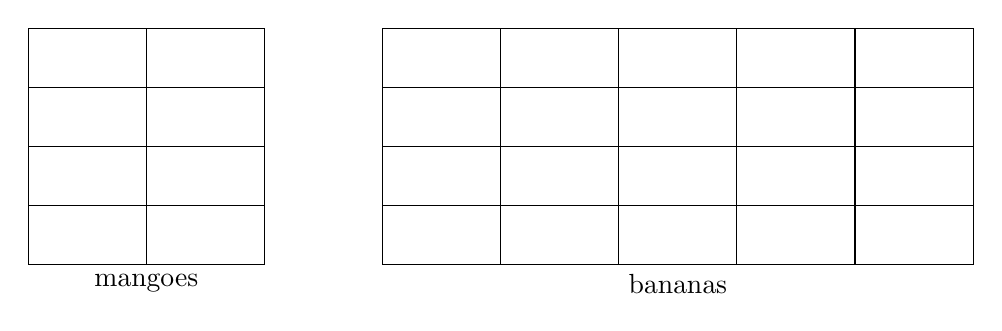
\begin{tikzpicture}[xscale=1.5,yscale=0.75]
\foreach \x in {0,1}
	\foreach \y in {0,1,2,3}
		\draw (\x,\y) rectangle +(1,1);
\node at (1,0) [below] {mangoes};
\begin{scope}[xshift=3cm]
\foreach \x in {0,1,2,3,4}
	\foreach \y in {0,1,2,3}
		\draw (\x,\y) rectangle +(1,1);
\node at (2.5,0) [below] {bananas};
\end{scope}
\end{tikzpicture}

Now from this diagram, we can take away 3/4 of the mangoes.

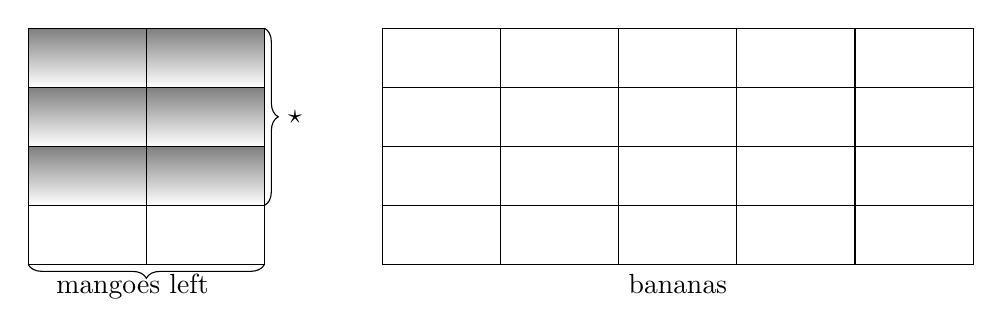
\begin{tikzpicture}[xscale=1.5,yscale=0.75]
\foreach \x in {0,1}
	\draw (\x,0) rectangle +(1,1);
\foreach \x in {0,1}
	\foreach \y in {1,2,3}
		\shadedraw [black,draw=black] (\x,\y) rectangle +(1,1);
\draw [decoration={brace,amplitude=5pt},decorate] (2,0) -- (0,0) node [below,pos=0.5,xshift=-5pt,align=center] {mangoes left};
\draw [decoration={brace,amplitude=5pt},decorate] (2,4) -- (2,1) node [right,xshift=5pt,pos=0.5,align=center] {$\fontsize{24}{24}\star\selectfont$};
\begin{scope}[xshift=3cm]
\foreach \x in {0,1,2,3,4}
	\foreach \y in {0,1,2,3}
		\draw (\x,\y) rectangle +(1,1);
\node at (2.5,0) [below] {bananas};
\end{scope}
\end{tikzpicture}

$\star$ mangoes given to her niece

Now how do we represent the 34 bananas given to her nephew? Take note that each of the
individual rectangle does not correspond to 1 banana. But we know that after giving the 34 bananas,
Mrs. Evangelista was left with mangoes and bananas in the ratio 2:3. Therefore, from the 20
rectangles of the bananas we can take away 17 of them so she's left with the ratio 2:3.

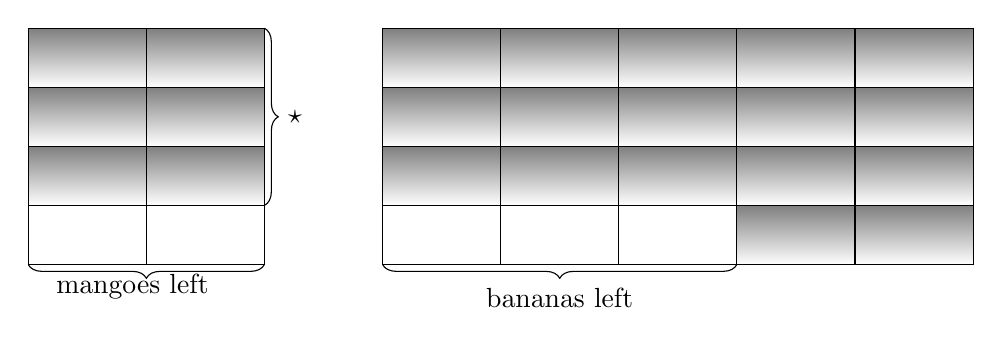
\begin{tikzpicture}[xscale=1.5,yscale=0.75]
\foreach \x in {0,1}
	\draw (\x,0) rectangle +(1,1);
\foreach \x in {0,1}
	\foreach \y in {1,2,3}
		\shadedraw [black,draw=black] (\x,\y) rectangle +(1,1);
\draw [decoration={brace,amplitude=5pt},decorate] (2,0) -- (0,0) node [below,pos=0.5,xshift=-5pt,align=center] {mangoes left};
\draw [decoration={brace,amplitude=5pt},decorate] (2,4) -- (2,1) node [right,xshift=5pt,pos=0.5,align=center] {$\fontsize{24}{24}\star\selectfont$};
\begin{scope}[xshift=3cm]
\foreach \x in {0,1,2}
	\draw (\x,0) rectangle +(1,1);
\foreach \x in {3,4}
	\shadedraw (\x,0) rectangle +(1,1);
\foreach \x in {0,1,2,3,4}
	\foreach \y in {1,2,3}
		\shadedraw [black,draw=black] (\x,\y) rectangle +(1,1);
\draw [decoration={brace,amplitude=5pt},decorate] (3,0) -- (0,0) node [below,pos=0.5,yshift=-5pt,align=center] {bananas left};
\end{scope}
\end{tikzpicture}

The 17 rectangles are equal to the 34 bananas given to his nephew, which means that each rectangle
represents 2 bananas. And each of the rectangles on the left represents 2 mangoes. From this, we
can conclude that originally, Mrs. Evangelista bought $16 (8 \times 2)$ mangoes and $40 (20 \times 2)$ bananas.

\Item Adia and Elijah had the same amount of money at first. When Adia gave Php 18 to Elijah,
Elijah then had five times as much money as his sister. How much money do Adia and Elijah have
together?

\Solution

Before Adia gave Php 18 to Elijah, They both have the same amount of money, which we can represent as follows:

\begin{tabular}[t]{m{1cm}l}
Adia: & \tikz [xscale=1.5,yscale=0.75] \draw (0,0) rectangle (3,1);\\
Elijah & \tikz [xscale=1.5,yscale=0.75] \draw (0,0) rectangle (3,1);\\
\end{tabular}

But after receiving Php 18 from his sister, Elijah had five times as much money as Adia.

\begin{tabular}[t]{m{1cm}l}
Adia: & \tikz [xscale=1.5,yscale=0.75] \draw (0,0) rectangle (1,1);\\
Elijah & \tikz [xscale=1.5,yscale=0.75] \foreach \x in {0,1,2,3,4} \draw (\x,0) rectangle +(1,1);\\
\end{tabular}

Notice that if we move the two blocks from Elijah's to Adia's, they will have the same number of
blocks. This implies that the two blocks are equivalent to the Php 18 that Adia gave to Elijah.
Therefore,
\begin{align*}
\tikz [baseline={([yshift=-3pt]current bounding box.center)},xscale=1.5,yscale=0.75] \foreach \x in {0,1} \draw (\x,0) rectangle +(1,1); &= \Php 18\\
\text{So}\quad \tikz [baseline={([yshift=-3pt]current bounding box.center)},xscale=1.5,yscale=0.75] \draw (0,0) rectangle (1,1); &= \Php 9
\end{align*}
Since they have a total of 6 blocks, $then 6(9) = 54$. Hence, Adia and Elijah have \Php{} 54 altogether.

Andres weigh 150 kg more than Balagtas. Cresencio weigh 130 kg less than Andres. Altogether the
three weigh 410 kg. What is the weight of Andres?
\end{example}

\section*{EXERCISES}
Answer the following problems using the block model.
\begin{enumerate}
\item One number is greater than half of another number by 15. What are the two numbers if
their sum is 48?
\item Mrs. Cruz is using the following recipe in making a juice cocktail: 1/2 cup of pineapple juice $+$ 3/4
cup of mango juice $+$ 1 1/4 cup of apple juice. She will be hosting a party this coming
Saturday. How much of each type of juice will she need if she wants to make 5 liters of this
juice cocktail?
\item A sum of money was divided among Elena, Felicisima, and Gracia in the ratio 2:4:5. Had the
sum of money been equally divided among them, Elena's share would have been larger by
Php 3000. What was the total sum of money?
\item Ben and Caloy are coin collectors. Initially 1/5 of Caloy's coins were equal to 1/3 of Ben's
coins. If Ben gave 24 coins to Caloy, Caloy would have thrice as many coins as Ben. How
many coins did each of them have originally?
\end{enumerate}

\section*{SUGGESTED ACTIVITY}
The participants are tasked to create/design your own word problems (3 word problems
each) using the block model. The level of difficulty of the problems should be easy, average and
difficult. Make sure to have your solution for each of the problem. Write your word problems and
the corresponding solutions to the papers provided for you. You are given 1 1/2 hours to accomplish
the task. After which, some of you will be asked to present his/her output to the rest of the
participants.
